This section outlines the experimental setup, covering the task definition, dataset, and models used. It begins with an introduction to the task and dataset, followed by a detailed description of the models employed. The section then discusses the conducted experiments and concludes with an analysis of the obtained results.

\subsection{Overview: Task, Dataset, and Models}

\paragraph{Task Definition.}
The task setup follows the \textit{SemEval 2024 Task 9: BrainTeaser}~\cite{jiangBRAINTEASERLateralThinking2023} challenge, simulating a participant's approach but with the constraint of using \acp{oLLM}. This contrasts with the original competition, where most participants (90\%) relied on closed-source models, such as \acs{GPT}-4~\cite{openaiGPT4TechnicalReport2024}, \acs{GPT}-3.5, and Gemini Pro~\cite{teamGeminiFamilyHighly2024}. As in the official task, evaluation follows a direct question-answering format: each model receives a puzzle question and must generate the correct answer from a provided list. To improve model performance, prompt optimization techniques such as \ac{ICL}~\cite{brownLanguageModelsAre2020} are applied, including additional strategies like instructing the model to \textit{"think outside the box"} or \textit{"think step by step"}. No fine-tuning is performed, instead, the focus is on leveraging prompting techniques.

\paragraph{Dataset.}
Experiments are conducted on the dataset from \citewithtitle{jiangBRAINTEASERLateralThinking2023}, publicly available on \hreffootnote{https://github.com/1171-jpg/BrainTeaser}{GitHub}. It consists of 1,100 lateral thinking puzzles formatted as question-answer pairs. The puzzles are categorized into \textit{Sentence Puzzles}, which challenge commonsense expectations based on sentence structures, and \textit{Word Puzzles}, where the answer defies the default meaning of a word and instead focuses on its letter composition~\cite{jiangBRAINTEASERLateralThinking2023}. Additionally, the puzzles are grouped into sets that include the original questions and their semantic and contextual variations, allowing for a systematic assessment of model consistency across different formulations~\cite{jiangBRAINTEASERLateralThinking2023}.

While \textit{SemEval 2024 Task 9} offers an alternative dataset with a predefined training-evaluation split, this experiment follows the original study~\cite{jiangBRAINTEASERLateralThinking2023}, evaluating \acp{LLM} on the full dataset.

\paragraph{Model selection.}
Experiments are conducted using the following open-source and open-weight models: \ac{LLaMA} 3.1 and 3.2~\cite{grattafioriLlama3Herd2024}, \acs{Phi} 3.5 and 4~\cite{abdinPhi3TechnicalReport2024, abdinPhi4TechnicalReport2024}, \acs{Qwen}~\cite{qwenQwen25TechnicalReport2025}, \acs{Gemma}~\cite{teamGemma2Improving2024}, and \acs{Mistral}~\cite{MistralNeMoMistral}. These models were selected for their open-source or open-weight nature, ensuring public access to their source code and/or model weights, as well as for their state-of-the-art performance in reasoning and problem-solving tasks~\cite{grattafioriLlama3Herd2024, abdinPhi3TechnicalReport2024, abdinPhi4TechnicalReport2024, qwenQwen25TechnicalReport2025, teamGemma2Improving2024, MistralNeMoMistral}.

Each model was evaluated across all available parameter sizes that fit within the 24 GB \ac{VRAM} of an NVIDIA GeForce RTX 3090. For smaller models (fewer than 3B parameters), FP16 precision was used due to their sensitivity to quantization, which reduces the precision of weights and activations~\cite{liEvaluatingQuantizedLarge2024}. For models up to 14B parameters, Q8\_0 precision was applied where possible, as recent studies suggest no significant performance difference between FP16 and Q8\_0~\cite{raubaQuantifyingPerturbationImpacts2024, liEvaluatingQuantizedLarge2024}. Models with over 27B parameters were evaluated using Q4\_K\_M precision to fit within \ac{VRAM}.

\paragraph{Evaluation Metrics.}
\label{evaluation-metrics}
Model performance is assessed using three accuracy metrics from \textcite{jiangBRAINTEASERLateralThinking2023}: \textit{(1) Instance-based Accuracy}, which measures performance on individual puzzles; \textit{(2) Group-based Accuracy}, which evaluates consistency across the original puzzle and its variations, awarding a score of 1 only if all variations are correctly solved; and \textit{(3) Overall Accuracy}, which reflects accuracy across all instances.

Metrics are reported for both \textit{raw} and \textit{processed} model responses. A \textit{raw response} refers to the model's direct output, where the answer is checked for an exact match with the expected choice or text. A \textit{processed response} involves applying advanced techniques to extract the answer from potentially verbose text, i.e., in cases where the model response includes additional text or prefixes before the answer itself, such as \textit{"Based on the evaluation of all choices, the best choice is (A)"}.

\paragraph{Prompt}
For all experiments, a modified version (cf.~\Cref{fig:prompt-template}) of the original prompt from \textcite{jiangBRAINTEASERLateralThinking2023} is used. The placeholders, i.e.,\{question\}, enclosed in curly braces, are replaced with specific content, e.g., \textit{"What part of London is in France?"}, during the experiments.

\begin{figure}[htb]
  \centering
  \fcolorbox{blue}{white}{
    \parbox{0.97\textwidth}{
      \centering
      Please select the best answer for the question. Each question has only one correct answer, including the choice 'None of above'. Your answer should only include the choice:\\

      Question: \{question\}
      \\
      Choice:
      \\
      (A) \{choice1\}
      (B) \{choice2\}
      (C) \{choice3\}
      (D) None of above
      \\
      Answer:
    }%
  }
  \caption[Example of the modified model prompt template, based on the original prompt from \textcite{jiangBRAINTEASERLateralThinking2023}]{Example of the modified model prompt template, based on the original prompt from \textcite{jiangBRAINTEASERLateralThinking2023}. The term \textit{"brain teaser"} was replaced with \textit{"question"} to align with standard terminology, and the option \textit{"none of the above"} was enclosed in quotes to ensure the model recognizes it as a selectable choice.}
  \label{fig:prompt-template}
\end{figure}

\subsection{Experiments}

Four experiments were conducted to evaluate the impact of different prompts on model performance. The experiments consist of two primary variations: one using the default system prompt and the other incorporating a lateral thinking variation to see if it provided any advantage.

\paragraph{Zero-Shot Baseline.}
\label{sec:zero-shot-prompt}

Each \ac{LLM} is evaluated in a zero-shot setting using the default system prompt: \textit{"You are a helpful AI assistant"}. A system prompt is a general instruction given to the model before the actual user prompt to guide its behavior. Normally, such a prompt could provide basic guidance, but in this experiment, the string does not include additional instructions or examples. As a result, the model relies solely on its pre-trained knowledge to generate responses.

\paragraph{Zero-Shot with Prompt Engineering.}
\label{sec:zero-shot-prompt-engineering}

Building on the \nameref{sec:zero-shot-prompt} experiment, 12 different system prompts are tested, each designed to encourage lateral thinking. These prompts include instructions such as \textit{"You are \{...\}. Think step by step \{...\}"} or \textit{"\{...\} consider hidden meanings and metaphorical interpretations {...}"}. Each system prompt ($s_i$) is applied to every model ($m_i$) on a 10\% random split of the dataset. The best-performing prompt for each model is then selected. This $s_i$ is added before the user prompt, and the model is evaluated on the entire dataset.

\paragraph{Few-Shot Prompting}
\label{sec:few-shot-prompt}

This experiment utilizes \acf{ICL}~\cite{brownLanguageModelsAre2020}, i.e., $n$-few-shot prompting, to improve model performance. Few-shot prompting involves presenting a constrained set of examples within the prompt to aid \acl{ICL} and guide the model's response generation~\cite{brownLanguageModelsAre2020}. For chat-based models, examples are primarily provided in a conversational form, i.e., a chat history $H = ((u_1, a_1), (u_2, a_2), \ldots, (u_n, a_n), u_p)$~\cite{HowUseFew}, where each example $e_i = (u_i, a_i)$ consists of a user prompt ($u_i$) and the corresponding answer ($a_i$). The final user query of interest ($u_p$) is inserted as the last item in $H$. This $H$ is then supplied to the model as input.

To reduce bias, such as the model favoring a particular answer choice due to its frequency in $H$, examples are randomly selected while maintaining diversity in answer labels where possible. The optimal number of examples ($n_i$) for each model ($m_i$) is determined by testing $n \in [1, 8]$ on a random 10\% subset of the data, as running all values on the full dataset would be too costly and time-intensive. The results of this initial experiment then guides the selection of an optimal $n_i$ for each model, and each model is prompted with its respective $n_i$ on the full dataset.

\paragraph{Few-Shot with Prompt Engineering.}
\label{sec:few-shot-optimized}

This experiment combines \nameref{sec:zero-shot-prompt-engineering} and \nameref{sec:few-shot-prompt}. As in the \nameref{sec:few-shot-prompt} experiment, examples are presented in a conversational format, integrating both user queries and correct responses before the final user query. The only change is the use of the best-performing system prompt ($s_i$) obtained in \nameref{sec:zero-shot-prompt-engineering}. Each model ($m_i$) is prompted with the optimal number of examples ($n_i$) and the best system prompt ($s_i$) obtained from the zero-shot experiments.

%%%%%%%%%%%%%%%%%%%%%%%%%%%%%%%%%%%%%%%%%%%%%%%%%%%%%%%%%%%%%
%%                        Results                          %%
%%%%%%%%%%%%%%%%%%%%%%%%%%%%%%%%%%%%%%%%%%%%%%%%%%%%%%%%%%%%%
\subsection{Results}

This section examines three key questions: (1) the raw performance of \ac{oLLM} across all experimental settings, (2) the effect of postprocessing on performance, and (3) how the best-performing model compares to other predominantly closed \acp{LLM} in the \textit{SemEval}~\cite{jiangSemEval2024Task92024} competition.
\smallbreak
For clarity, \acs{SP} and \acs{WP} performance scores refer to the overall accuracy on the \acf{WP} and \acf{SP} subsets, respectively.

\subsubsection{Performance across Experiments}
\label{sec:performance-across-experiments}

The main results of all experiments are summarized in \Cref{tab:baseline-vs-optimized-zero-shot-raw,tab:baseline-zero-shot-vs-baseline-few-shot-raw,tab:baseline-vs-optimized-few-shot-raw}. To gain insights into how the models performed and how \acf{ICL} and prompt engineering applied to the system prompt influenced the results, the tables are discussed sequentially. Additionally, \Cref{tab:full-zero-shot,tab:full-few-shot,tab:optimized-zero-shot-vs-optimized-few-shot}, containing both raw and postprocessed results, are included but not discussed in detail.

\paragraph{Zero-Shot}
\label{par:zero-shot}

\Cref{tab:baseline-vs-optimized-zero-shot-raw} presents the results from the \nameref{sec:zero-shot-prompt} and \nameref{sec:zero-shot-prompt-engineering} experiments. In the baseline experiment, approximately half of the models outperform the random guesser. Smaller models, such as LLaMa 3.2, Phi 3.5, QWEN2.5, and the Gemma2 variants with fewer than 7B parameters, tend to underperform, failing to exceed random guesser performance on both the \ac{SP} and \ac{WP} subsets. Only four out of 15 models surpass 50\% accuracy on \ac{SP}, and none exceed 50\% on \ac{WP}. The best-performing model, Gemma2:9B, achieves 68.10\% and 47.36\% on \ac{SP} and \ac{WP}, respectively.

Interestingly, models perform significantly better on \ac{SP} than on \ac{WP}. However, this is not entirely surprising, as \ac{SP} is dominated by topics related to math, physics, and nature, whereas \ac{WP} is primarily language-based~\cite{jiangBRAINTEASERLateralThinking2023}. Given the trend in previous research and model tuning favoring predominantly vertical thinking tasks, such as math~\cite{jiangBRAINTEASERLateralThinking2023,jiangSemEval2024Task92024}, I hypothesize that models struggle with \ac{WP} due to suboptimal optimization for language-related topics. Additionally, violations of the default meanings of words within the \ac{WP} subset likely further mislead models into disproportionately favoring option \textit{"(D) None of the above"}, even though it is rarely the correct answer.

In the \nameref{sec:zero-shot-prompt-engineering} experiment, performance systematically decreases by 3.68\% and 5.81\% compared to the baseline, with QWEN2.5:32B being the best-performing model at 65.55\% and 54.27\% for \ac{SP} and \ac{WP}. I hypothesize that this performance drop is primarily due to the excessive auxiliary text generated by the models, which negatively impacts the raw results. To address this, I examined the postprocessed results, which aim to extract the model's intended answer. Postprocessing shows that this hypothesis holds, as performance increases by 7.15\% on \ac{SP} and 8.89\% on \ac{WP} after applying postprocessing to the models' responses (cf.~\Cref{tab:full-zero-shot}).

Interestingly, while postprocessing results show substantial performance gains, smaller models continue to mostly fail to surpass random guesser performance, although they are catching up. After reviewing these models specifically, it becomes clear that the postprocessing does not capture all auxiliary text variants, as manual examination of a few examples showed incorrect answer extraction. Thus, it would be interesting to improve the postprocessing algorithm and then re-evaluate the results. On the other hand, larger models demonstrate significant improvements, with some achieving modest performance gains in the single-digit to low double-digit range, without requiring further tweaking of the postprocessing algorithm. Notably, QWEN2.5:32B shows the largest improvements from prompt engineering, with raw gains of 16.59\% and 29.88\%, respectively.

\paragraph{Few-Shot}
\label{par:few-shot}

\Cref{tab:baseline-zero-shot-vs-baseline-few-shot-raw} presents the results of the \nameref{sec:zero-shot-prompt} and \nameref{sec:few-shot-prompt} experiments. The results show that few-shot prompting significantly enhances model performance, with an average increase of 20.23\% on \ac{SP} and 23.38\% on \ac{WP} in raw overall performance. When comparing postprocessed model results, the increase remains substantial at 14.56\% on \ac{SP} and 20.44\% n \ac{WP} (cf.~\cref{tab:full-few-shot}). Compared to zero-shot, nine out of 15 models now exceed 50\% performance on \ac{SP}, while four out of 15 surpass 50\% on \ac{WP}. These improvements are particularly notable, as they reflect consistent gains across multiple models rather than being driven by a few exceptional cases, highlighting the overall benefits of few-shot prompting.

When comparing this technique to the prompt engineering experiment, smaller models also see substantial improvements with few-shot prompting. Previously, no smaller models (with fewer than 7B parameters) exceeded random guesser performance (24.04\% on \ac{SP} and 25.34\% on \ac{WP}). However, with few-shot prompting, these models now achieve average performances of 31.36\% on \ac{SP} and 31.72\% on \ac{WP}, respectively. Larger models also show significant improvements, with the top-performing models now being Phi4:14B (77.72\% and 69.53\%) and Gemma2:27B (79.81\% and 64.83\%), surpassing the previously best-performing model, Gemma2:9B, from the zero-shot setting.

At this stage, the question arises as to whether few-shot prompting is more effective at eliciting information from the models compared to prompt optimization, or if the observed performance improvements could be primarily due to the models now having a clearer understanding of the expected output format. To investigate this, a manual inspection of model responses was performed, which revealed that, with few-shot prompting, most models now consistently output in the required format, avoiding the auxiliary text present in the zero-shot baseline. This suggests that the lower performance observed in the system prompt-optimized zero-shot experiment may indeed have been due to output format inconsistencies rather than a lack of model knowledge. A further evaluation of the \nameref{sec:few-shot-optimized} experiment could provide more clarity on this matter.

\paragraph{Few-Shot with Optimized System Prompt}

\Cref{tab:baseline-vs-optimized-few-shot-raw} compares the results of the baseline and system prompt-optimized few-shot experiment. As hypothesized in the \nameref{par:few-shot} analysis, combining both techniques improves performance by 6.06\% over baseline few-shot on \ac{SP}, while resulting in a 5.48\% decrease on \ac{WP} (cf.~\Cref{tab:full-few-shot}). This tendency to decrease performance was already observed in the analysis of the \nameref{par:zero-shot} experiment, where prompt engineering worsened raw performance, while postprocessing led to significant improvements. The same trend is observed here, where postprocessed results show a 6.27\% improvement for \ac{SP} and 0.05\% for \ac{WP}.

Although combining both techniques results in a combined 0.58\% raw performance improvement, this modest increase is likely due to run-to-run variations or model instability. Therefore, rerunning the experiment across multiple runs and adjusting parameters such as model seed and temperature could provide greater clarity and enable a more accurate evaluation of the benefits of combining both techniques. Nonetheless, this slight increase was sufficient to push Phi4:14B out, with the best models now being Gemma2:27B (80.45\% and 67.28\%) and Gemma2:9B (76.76\% and 66.87\%).

\paragraph{Conclusion}

The overall results show that models tend to perform significantly better on \ac{SP} than on \ac{WP}. For example, the best-performing model, Gemma2:27B, achieved 80.45\% on \ac{SP} and 67.28\% on \ac{WP}. I hypothesize that the dominance of math- and science-related content in \ac{SP}, as opposed to the more nuanced language reasoning required for \ac{WP}, likely contributes to this performance gap~\cite{jiangBRAINTEASERLateralThinking2023}. Prior research and model tuning favoring vertical thinking tasks~\cite{jiangSemEval2024Task92024} may also play a role.

Few-shot prompting improves performance, particularly for larger models, while smaller models continue to face challenges. Specifically, few-shot prompting yields gains of 20.23\% for \ac{SP} and 23.38\% for \ac{WP} in raw performance. System prompt optimization, on the other hand, leads to decreases of 3.68\% for \ac{SP} and 5.81\% for \ac{WP} due to additional auxiliary text, although postprocessing helps recover some accuracy. When combining few-shot prompting with system prompt optimization, performance improves by 6.06\% for \ac{SP}, while \ac{WP} experiences a 5.48\% decrease. These findings suggest that few-shot prompting alone may be more effective in terms of raw performance, as the combined approach yields only modest improvements of 0.58\%, likely due to noise.

\subsubsection{Implications of Raw vs. Postprocessed Performance}
\label{par:raw-vs-post-performance}

As highlighted in the previous section, system prompt optimization can negatively impact raw performance despite leading to substantial gains after postprocessing model responses. With insights from \Cref{sec:performance-across-experiments}, this pattern is evident in both zero-shot and few-shot experiments, where prompt engineering initially reduces raw accuracy but improves results once auxiliary text is accounted for.

Raw performance metrics do not consider auxiliary text, which often arises when applying prompt engineering techniques, such as instructing the model to \textit{Think Step-By-Step}. This additional text is the primary factor lowering raw scores, even when the actual answers remain correct. Consequently, if one were to rely solely on raw performance, it would appear that prompt engineering, on average, decreases accuracy, while few-shot prompting significantly enhances it.

When considering postprocessed results, both prompt engineering and few-shot prompting significantly improve performance by 7.15\% on \ac{SP} and 8.89\% on \ac{WP}, increasing to 14.56\% and 20.44\%, respectively, when postprocessing is applied. Moreover, combining both techniques leads to improvements in both raw and postprocessed metrics, with gains of approximately 1.9\% in raw performance and 6.33\% in postprocessed performance over the baseline few-shot.

These findings underscore the importance of evaluating model outputs beyond the raw performance metric alone. Relying exclusively on raw model response evaluations can lead to misleading conclusions, as models may generate correct answers but with excessive verbosity. Although a more in-depth analysis was beyond the scope of this paper, the results suggest that developing methods to extract correct responses from verbose outputs would be highly beneficial. This is particularly relevant in applications where correctness takes precedence over strict format adherence.

\subsubsection{Performance Comparison with SemEval Participants}

The best-performing model in this paper, Gemma2:27B-(SPO-FS\footnote{SPO-FS refers to \underline{S}ystem-\underline{P}rompt-\underline{O}ptimized \underline{F}ew-\underline{S}hot Prompting}), achieves 80.45\% overall accuracy on \acf{SP} and 67.28\% on \acf{WP} tasks, respectively. This would have ranked 15th out of 30 on \ac{SP} and approximately 16th on \ac{WP} on the \href{https://brainteasersem.github.io/\#leaderboard}{SemEval leaderboard}.

When checking closed-source models, such as GPT-4~\cite{openaiGPT4TechnicalReport2024}, the leaderboard shows strong performance (above 90\%) on both \ac{SP} and \ac{WP} (Figure 4 by \textcite{jiangSemEval2024Task92024}). However, a deeper dive reveals that these results were achieved by leveraging more advanced techniques. Many of the top submissions combined several optimization strategies to achieve such high scores, with few-shot prompting being a crucial component. For instance, some teams identified particularly challenging puzzle instances in the training set and employed methods like \ac{CoT} (Chain-of-Thought) to generate rationales for both correct and incorrect answers, which were then included as few-shot examples for the prompt. Other teams adjusted the model's temperature to control the level of randomness in the model's responses, which helped enhance performance. In general, they also used larger models (i.e., GPT-4), referring to the number of parameters, which is comparable to LLaMa 3 (405B), which in turn outperforms the here tested models significantly~\cite{grattafioriLlama3Herd2024, openaiGPT4TechnicalReport2024}.

Considering these factors, it is reasonable to conclude that the \acp{oLLM} evaluated in the experiments, such as Phi4 and Gemma2, achieved competitive performance in \textit{SemEval 2024 Task 4: BrainTeaser} without relying on advanced techniques like \ac{CoT}, cherry-picked examples for few-shot prompting, or opting for larger parameter-count counterparts.

\subsubsection{Interference speeds}
\begin{figure}[H]
  \centering
  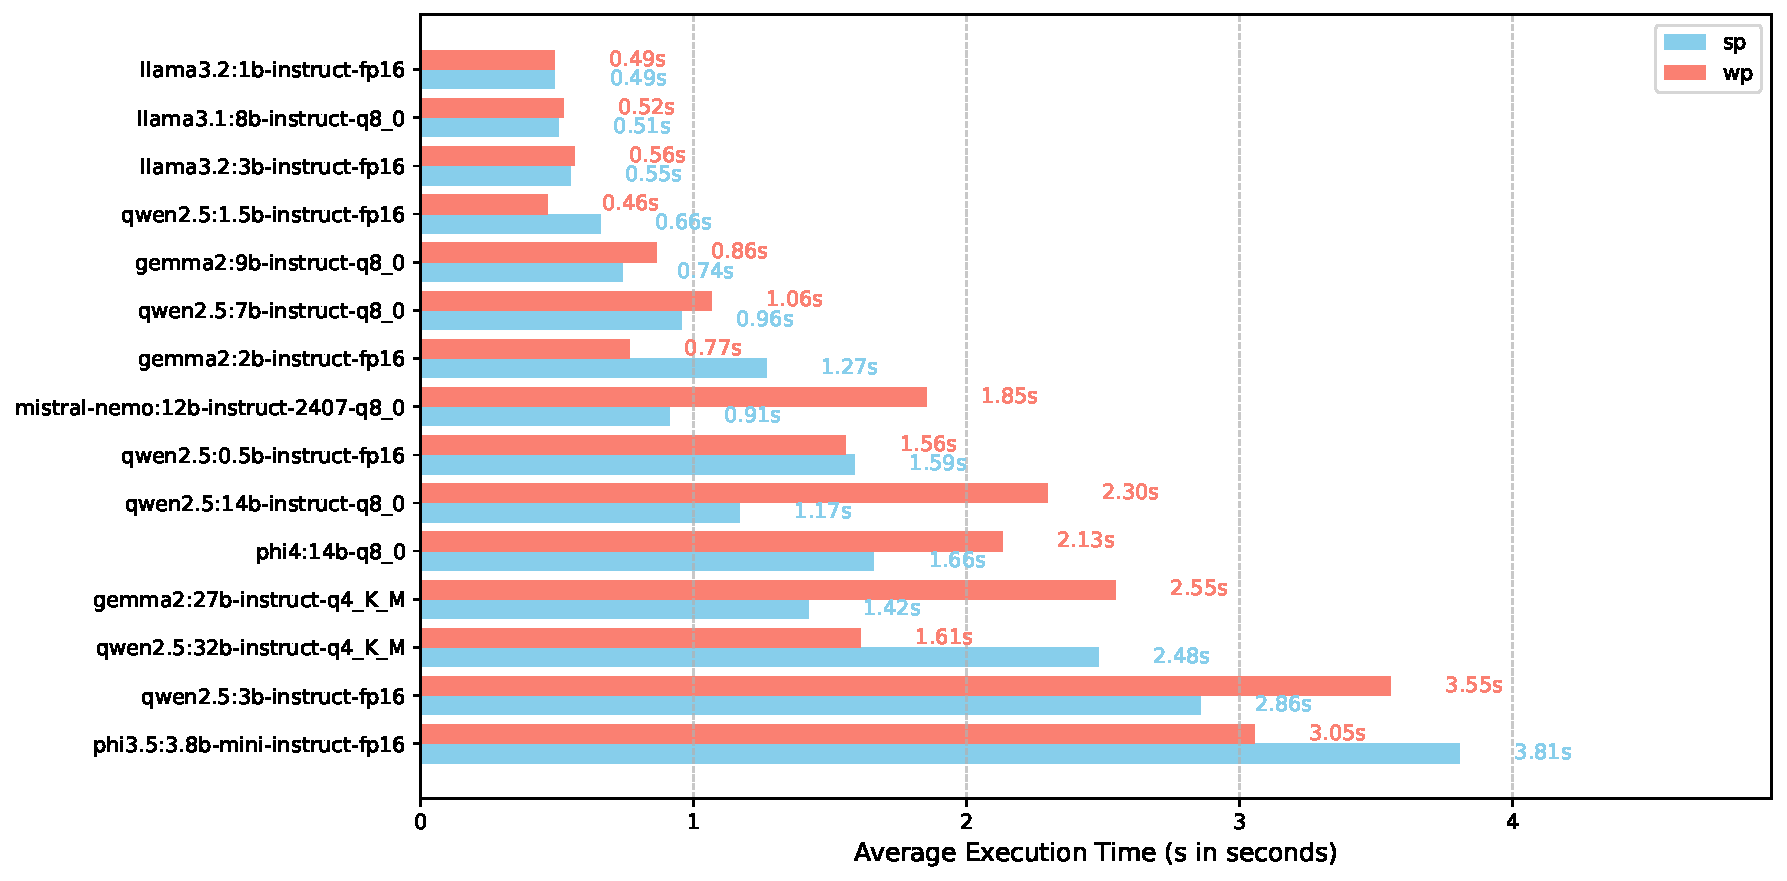
\includegraphics[width=0.8\linewidth,keepaspectratio]{assets/plots/execution-times.pdf}
  \caption[Average Execution Times for Models Across All Experiments by Dataset in Seconds]{Average Execution Times for Models Across All Experiments by Dataset (in Seconds). 'Blue' bars refer to \aclp{SP}, while 'Red' bars refer to \aclp{WP}.}
  \label{fig:interference}
\end{figure}

The interference speeds across models (cf.~\Cref{fig:interference}) show little variation, especially when considering the \ac{VRAM} requirements. The LLaMA family is the fastest, with nearly no difference in processing speed between SP and WP conditions or across different parameter sizes. In contrast, Phi3.5:3.8B is the slowest with 3.43s, taking significantly more time despite its relatively small size. Other models generally show consistent scaling, with larger models taking longer to process.

Interestingly, QWEN2.5:3B is notably slow for no apparent reason, as its 7B variant only takes around 1 second. Additionally, most models require more time on WP than SP, which is unexpected since WP contains shorter text instances compared to SP. This could be due to the increased reasoning required by WP, due to more complex word meanings, potentially distracting the models.

However, since the experiments were conducted on a shared system, these results should be interpreted with caution. It would have been ideal to benchmark all models using the same seed across multiple runs to ensure fairness, as the seed could have impacted the interference performance.